\chapter{Phương pháp giải quyết}
Ở chương này, chúng ta sẽ phân tích các vấn đề cụ thể trong đề tài và đưa ra lựa chọn giải quyết cần thiết.\par 
\section{Phân tích}
	\subsection{Mô tả tập dữ liệu}
	Một trong những vấn đề cần được quan nhất trong đề tài này chính là đặc điểm của tập dữ liệu. Sau một khoảng thời gian truy xuất video lấy từ camera hành trình, chúng ta có được khoảng hơn 14000 ảnh về giao thông. Theo như đã tìm hiểu và so sánh, có thể thấy đây không phải là một tập ảnh lớn nếu so với tập dữ liệu IgmageNet gồm khoảng 14 triệu ảnh thuộc 1000 lớp khác nhau. Ngoài ra, các ảnh thu được từ camera hành trình thật chất không phải là bộ ảnh có chất lượng tốt.\par 
	Toàn bộ số ảnh trên được thực hiện gán nhãn dựa trên hai nhãn chính là kẹt và thông thoáng để phục vụ cho việc huấn luyện. Dưới đây là một số hình ảnh được trích ra từ tập ảnh. Với hai hình đầu được lấy ra từ lớp thông thoáng, hai hình sau được lấy ra từ lớp ùn tắt.
	\begin{figure}[h!]
  \centering
  \begin{subfigure}[b]{0.4\linewidth}
    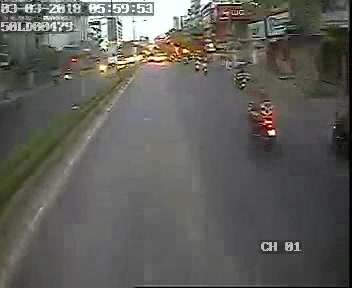
\includegraphics[width=\linewidth]{charts/image0125.jpg}
    \caption{Ảnh mẫu 1}
  \end{subfigure}
  \begin{subfigure}[b]{0.4\linewidth}
    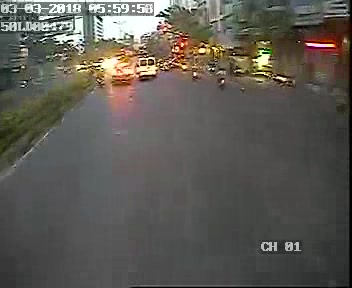
\includegraphics[width=\linewidth]{charts/image0126.jpg}
    \caption{Ảnh mẫu 2}
  \end{subfigure}
  \label{fig:sample1}
  \caption{Ảnh mẫu trong phân lớp thông thoáng}
\end{figure}

\begin{figure}[h!]
  \centering
  \begin{subfigure}[b]{0.4\linewidth}
    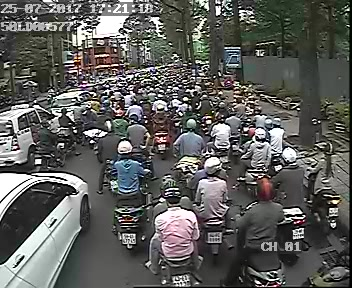
\includegraphics[width=\linewidth]{charts/test-ket.jpg}
    \caption{Ảnh mẫu 3}
  \end{subfigure}
  \begin{subfigure}[b]{0.4\linewidth}
    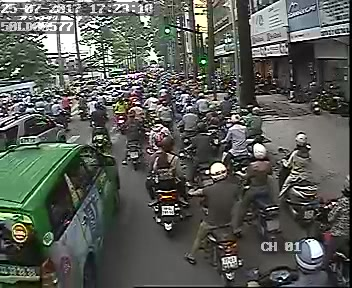
\includegraphics[width=\linewidth]{charts/test-ket1.jpg}
    \caption{Ảnh mẫu 4}
  \end{subfigure}
  \label{fig:sample2}
  \caption{Ảnh mẫu trong phân lớp ùn tắt}
\end{figure}

	\subsection{Các vấn đề về lưu trữ}
	Trong đề tài này, ta cần thực hiện mô phỏng lại một hệ thống lưu trữ các dữ liệu ghi nhận từ xe buýt đang hoạt động. Các dữ liệu này bao gồm các video được ghi lại từ các camera hành trình trên xe buýt và dữ liệu GPS mà xe buýt đó gửi về liên tục.\par 	

\section{Giải pháp đề xuất}
	\subsection{Kiến trúc mạng googleNet}
	Với tập dữ liệu có kích thước không lớn việc xây dựng một mạng neuron tích chập để huấn luyện sẽ dẫn đến kết quả phân loại không tốt và có thể tốn kém thời gian nếu không có cấu hình đủ mạnh để thực hiện. Chính vì vậy, việc sử dụng phương pháp transfer learning là lựa chọn cần thiết.
	\subsubsection{Phương pháp transfer learning}
	Ở các nội dung trước, ta đã trình bày cấu trúc của một mạng neuron tích chập bao gồm rất nhiều layers. Các layers đứng trước bao gồm nhiều tầng tích chập kết hợp với các hàm activation phi tuyến tính và các tầng tổng hợp. Tầng cuối cùng là một tầng kết nối đầy đủ (Fully Connected Layer) và thường là một hàm softmax, số lượng node (unit) ở tầng này bằng với số lượng lớp(label) cần phân loại. Vì thế ta đầu ra ở layer trước tầng cuối cùng là các vector đặc trưng (feature vector). Việc huấn luyện sử dụng mô hình gồm nhiều lớp như trên với một tập dữ liệu lớn khoảng hơn 1 triệu ảnh cũng tốn rất nhiều thời gian. Mà ở đây, chúng ta không có tập dữ liệu lớn như vậy và cũng không có thời gian quá nhiều. Vì thế, ta sử dụng một phương pháp là Transfer learning, sử dụng lại những mô hình sẵn có để áp dụng vào tập dữ liệu của chúng ta.\par 
	Để hiểu được phương pháp này, chúng ta nhìn lại, toàn bộ các lớp trong một mạng CNN được coi là bộ Feature Extractor. Dựa trên nhận xét rằng các bức ảnh đều có những đặc tính giống nhau nào đó, với cơ sở dữ liệu khác, ta cũng có thể sử dụng phần Feature Extractor này để tạo ra các feature vectors. Sau đó, ta thay output layer cũng bằng một Softmax Regression (hoặc multi-class SVM) nhưng với số lượng units bằng với số lượng class ở bộ cơ sở dữ liệu mới. Ta chỉ cần train layer cuối cùng này. Kinh nghiệm thực tế của tôi cho thấy, việc làm này đã tăng kết quả phân lớp lên rất nhiều.
		
	\subsubsection{Kiến trúc mạng GoogLeNet}
	
	Đây là kiến trúc mạng tích chập với 22 tầng. GoogLeNet còn là quán quân của ILSVRC 2014 \cite{1}. Mạng googLeNet có cấu trúc mạng nằm trong mạng, có 9 tầng mà mỗi tầng là một inception module. Theo tài liệu cho biết, việc áp dụng inception module giúp làm giảm đáng kể số lượng tham số tính toán giúp giải quyết vấn đề về tài nguyên. \ref{fig:googlenet} minh họa cho cấu trúc của mạng googLeNet.
	
		
	\begin{figure}[h!]
			\centering
			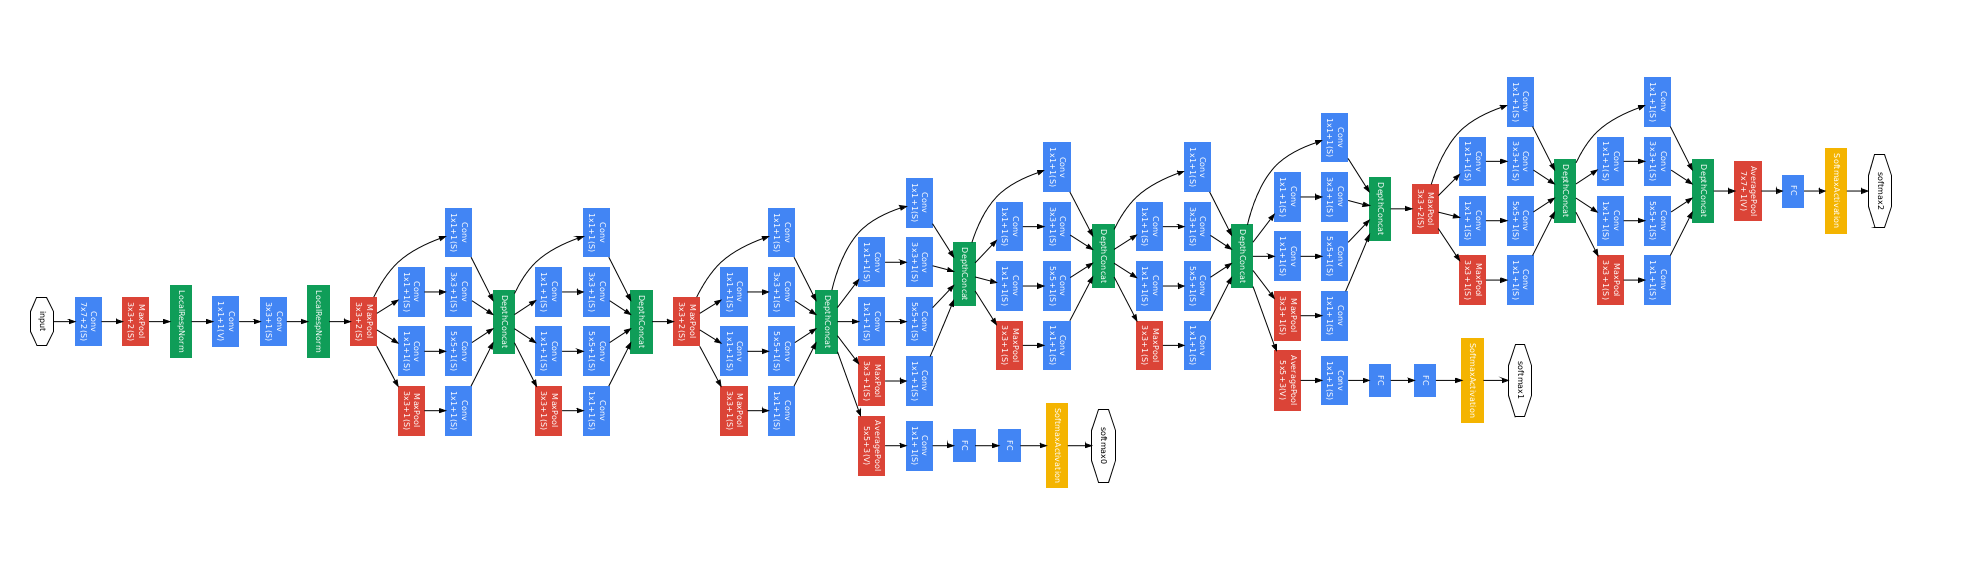
\includegraphics[scale=0.7]{charts/googlenet.png}
			\caption{GoogLeNet \cite{1}}
			\label{fig:googlenet}
		\end{figure}
		
	
	\textbf{Inception module}\\
	Với minh họa kiến trúc của mạng googLeNet, ta sẽ thấy các layer là một khối mạng nhỏ nằm bên trong. Đây là các inception module. Đối với các mạng tích chập thông thường, khi một tập dữ liệu bắt đầu đi vào một tầng thì sẽ chỉ có hai sự lựa chọn đó chính là tầng tích chập hoặc tầng tổng hợp, nhưng với googLeNet sẽ có tập input sẽ đi vào một lớp module tại đó sẽ các phương thức tích chập và pooling sẽ đươc tính toán một cách song song và độc lập với nhau \cite{1}.
	
	\begin{figure}[h!]
			\centering
			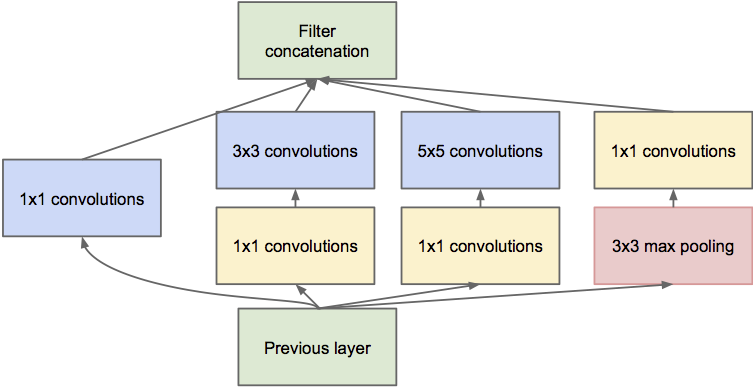
\includegraphics[scale=1.5]{charts/inception.png}
			\caption{inception module \cite{1}}
			\label{fig:inception}
	\end{figure}

	\begin{figure}[h!]
			\centering
			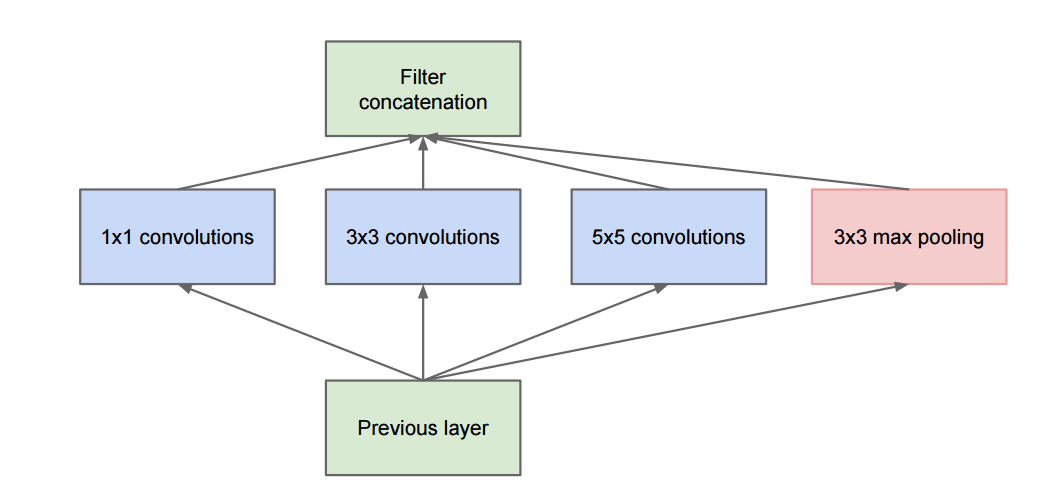
\includegraphics[scale=0.3]{charts/inception_nai.png}
			\caption{naive inception module \cite{1}}
			\label{fig:nai_inception}
	\end{figure}
	
	Hình \ref{fig:inception} miêu tả cấu trúc của một module trong mạng. Trong khi đó \ref{fig:nai_inception} là một ý tưởng ban đầu mà tác giả đã nghĩ tới. Ở \ref{fig:inception} chúng ta thấy trước khi thực hiện các phép tích chập với các filter 3 x 3 và 5 x 5, input đều được xử lý qua phép tích chập với filter 1 x 1. Các bộ lọc 1 x 1 có tác dụng làm giảm đi chiều của các input\cite{2}, điều này giúp cho khối lượng tham số phải tính toán ở phép toán tích chập với bộ lọc 3 x 3 và 5 x 5 sẽ được giảm đi một cách đáng kể.
	
	\subsection{Cấu trúc hệ thống lưu trữ}
	Để đáp ứng cho nhu cầu lưu trữ dữ liệu video và dữ liệu GPS này chúng ta có thể sử dụng Apache Hadoop kết hợp với HIVE.\par 
	Cấu trúc của hệ thống mô phỏng này sẽ bao gồm ba máy lưu trữ và một máy làm nhiệm vụ la máy chủ (master) để điều khiển hoạt động của các máy còn lại. Các video sẽ được lưu trữ theo từng thư mục, mỗi thư mục chứa dữ liệu các video trong một ngày đó.\par 
	Đối với HIVE, các dữ liệu GPS sẽ được lưu trữ trên một bảng dữ liệu của HIVE, bảng này bao gồm nhiều trường mô tả dữ liệu hoạt động của xe buýt, trong đó có các trường dữ liệu chính để chúng ta truy xuất như sau: Longtitude đây là kinh độ của xe buýt, Lattitude đây la vĩ độ của xe buýt, tracktime là dữ liệu thời gian có định dạng (YYYY-MM-DD hh-mm-ss). Như vậy, với một mẫu tin được lưu, sẽ thể hiện được thời gian cụ thể cũng như vị trí GPS của xe buýt tại thời gian đó.
